% TODO: FIX LATEX ERRORS
\chapter{Technische Grundlagen}
\section{\acf{OLAP}}
Viele Unternehmen verwenden heute große Mengen an Geschäftsdaten für eine strategische Planung.
Durch eine Analyse der Daten lassen sich Handlungsempfehlungen ableiten.
Typische Analysen umfassen die Berechnung des Umsatzes einer Filiale innerhalb des letzten Jahres sowie der Vergleich zu vorherigen Jahren oder die Analyse der Verkäufe von einzelnen Produkten in einem bestimmten Quartal.
Diese Analysen erfordern eine umfassende Datenmenge, einschließlich historischer Daten.
Klassische Datenbanksysteme für Transaktionen, etwa in einem Onlineshop, auch \acf{OLTP} genannt, sind für viele Schreib- und Lesezugriffe optimiert, nutzen meist wenig komplexe Abfragen (Queries) und enthalten häufig keine historischen Daten.
Datenbanken für analytische Zwecke sollten hingegen stark auf die Leseoperationen optimiert sein und müssen komplexere Queries in angemessener Zeit durchführen können.
Bei diesem Einsatzgebiet von Datenbanken spricht man vom \acf{OLAP}~\cite[S.~97f]{kleppmann_datenintensive_2019}.

\ac{OLAP} und \ac{OLTP} profitieren von verschiedenen Optimierungen der Datenstrukturen in einer Datenbank.
Bei Nutzung einer gemeinsamen Datenbank für beide Verfahren würden die \ac{OLAP}-Abfragen außerdem die \ac{OLTP}-Transaktionen verlangsamen oder blockieren.
Um das zu verhindern, nutzt man für \ac{OLAP} eigene Datenbanksysteme und speichert die Daten in sogenannten \acp{DW}.

\subsection{\acfp{DW}}
\acp{DW} wurden entwickelt, um Daten, die für strategische Entscheidungen im Geschäftsumfeld nützlich sein können, zu speichern.
Dazu werden Daten aus Geschäftsprozessen wie etwa Verkäufen extrahiert, für die weitere Verwendung transformiert und in bestimmten Datenbanken gespeichert.
Klassische  operative oder transaktionale Datenbankansätze, die auf den täglichen Gebrauch durch viele Nutzende optimiert sind, eignen sich nicht für ein \ac{DW} im \ac{OLAP}-Umfeld, da hier üblicherweise keine historischen Daten gespeichert werden.
Des Weiteren enthalten diese detaillierte Daten, was das Ausführen von komplexen Abfragen erschwert bzw. verlangsamt.
% Hier ähnliche Inhalte wie im Kapitel weiter oben
Um aber Entscheidungen aus den Daten ableiten zu können, sind sowohl historische Daten als auch komplexe Abfragen notwendig.
Um diese Probleme zu lösen, enthält ein \ac{DW} im \ac{OLAP} Umfeld historische Daten und bietet eine optimierte Datenstruktur für komplexere Abfragen.
In der ursprünglichen Definition nach Inmon werden \acp{DW} als Sammlung von subjektorientierten, integrierten, nicht flüchtigen und zeitvariablen Daten beschrieben. %Hier wäre Originalquelle ganz praktisch
Subjektorientiert bedeutet, dass sich die Daten auf bestimmte Aspekte der geforderten Analyse beziehen, also z.~B. Daten über Produktionsmengen und Verkäufen bei Produktionsunternehmen.
Mit integrierten Daten ist gemeint, dass Daten aus verschiedenen Umgebungen in dem \ac{DW} integriert sind.
Nicht flüchtig bedeutet, dass die Daten über lange Zeiträume hinweg gespeichert bleiben und somit weder gelöscht noch modifiziert werden.
Zur Analyse ist es wichtig, Daten im zeitlichen Verlauf miteinander zu vergleichen, etwa um herauszufinden, wie sich die Verkäufe im letzten Quartal entwickelt haben.
Zeitvariabel beschriebt daher, dass Daten aus verschiedenen Zeitpunkten gespeichert werden~\cite[S.~3f]{vaisman_data_2022}.

\subsection{Datenstruktur in Data Warehouses im \ac{OLAP} Umfeld}
Die Mehrheit der am häufigsten verwendeten Datenbanken nutzt ein relationales Datenbankmodell~\cite{db-engines_most_2023}. 
In einem solchen Modell können die Daten in verschiedenen Schemata aufgebaut sein.

\subsubsection{Normalisierung}
Eine gängige Praxis bei relationalen Datenbanken ist die Normalisierung.
Ziel der Normalisierung ist das Verhindern von redundanten Daten.
Enthalten mehrere Tabellen die gleichen Daten, so müssen diese Daten an mehreren Stellen bei Änderungen angepasst werden.
Um diesen Umstand zu verhindern, werden die Daten daher nur in einer Tabelle gespeichert und dann per Fremdschlüssel in den anderen Tabellen eingebunden~\cite[S.~24f]{vaisman_data_2022}.
Diese Fremdschlüssel benötigen in den meisten Fällen außerdem weniger Speicherplatz als die eigentlichen Daten, was einen weiteren Vorteil bietet.
Ein Nachteil der Normalisierung ist jedoch, dass Abfragen komplizierter werden und länger in der Ausführung benötigen, da die Daten aus verschiedenen Tabellen kombiniert werden müssen.

\subsubsection{Sternschema und Schneeflockenschema}
In \acp{DW}, die für große Datenmengen und komplexe Abfragen gedacht sind, bildet das Normalisieren durch die erschwerten Abfragen einen Nachteil.
Um Daten für Abfragen effizient zu speichern, werden diese nicht so weit wie möglich normalisiert, sondern anhand ihrer Inhalte verteilt. 
Durch Verständnis der Daten können diese in eine sogenannte Faktentabelle und viele Dimensionstabellen aufgeteilt werden.

In der Faktentabelle befinden sich die zentralen Metriken, die zur Analyse benötigt werden, etwa die Anzahl der Verkäufe eines Produktes.
Die Dimensionstabellen enthalten Daten, mit denen die Daten der Faktentabelle unter verschiedenen Umständen betrachtet werden können, etwa eine Dimensionstabelle mit Zeitpunkten oder Orten.
Diese Dimensionstabellen sind in der Faktentabelle verlinkt.

In einem Diagramm werden die Dimensionstabellen um die Faktentabelle angeordnet, wodurch das Diagramm einem Stern ähnelt, bei dem die Faktentabelle das Zentrum, und die Dimensionen die Strahlen bilden.
Deshalb spricht man auch von einem Sternschema.
Werden die Faktentabellen zusätzlich noch unterteilt, die Daten also noch normalisiert, spricht man von einem Schneeflockenschema.
Wie oben beschrieben eignen sich nicht normalisierte Daten jedoch besser für analytische Abfragen, weshalb das Sternschema oft bevorzugt wird.

Die Faktentabelle enthält den Großteil der Daten.
Jedes Ereignis wird in einer eigenen Zeile gespeichert, um somit so detailreich wie möglich analysieren zu können.
Des Weiteren kann die Faktentabelle sehr viele Spalten mit Details zu den Ereignissen enthalten.
Dimensionstabellen sind dahingegen wesentlich kleiner\cite[S.~101-103]{kleppmann_datenintensive_2019}.

Bei Abfragen können nun verschiedene Dimensionen kombiniert werden, um Daten aus der Faktentabelle abzufragen.
So können z.~B. die Verkäufe aus einem bestimmten Jahr in einer bestimmten Filiale aus der Faktentabelle abgefragt werden.
Die Dimensionstabellen können außerdem sogenannte Hierarchien enthalten, die verschiedene Genauigkeiten der Dimension definieren.
So kann ein Zeitpunkt in der Tabelle Werte für Uhrzeit, Tag, Monat, Quartal oder Jahr enthalten.
Ein Ort kann etwa aus dem Ortsnamen, dem Bundesland, dem Land, dem Kontinent bestehen.
So lassen sich genaue Abfragen zu Verkäufen einer bestimmten Filiale oder etwa allen Filialen in Europa abfragen~\cite[S.~5]{vaisman_data_2022}.

\begin{comment}
\subsection{Der OLAP-Cube}
%TODO: OLAP CUBE Voraggregation bei OLAP -> Kleppmann Seite 109 Kapitel 3


% Tabelle überdenken
\begin{table}[htbp] 
    \centering
    \footnotesize
    \begin{tabular}{ccccc}
        \toprule  
        Id & Umsatz & Stückzahl & Zeit & Ort \\
        \midrule
        1 & 100,00 € & 50 & 1 & 1 \\
        2 & 200,00 € & 100 & 2 & 2 \\
        3 & 150,00 € & 75 & 3 & 3 \\
        \bottomrule
    \end{tabular}
    \caption{Faktentabelle mit Umsatz, Stückzahl, Zeit und Ort}
    \label{tab:faktentabelle}
\end{table}

\begin{table}[htbp] 
    \centering
    \footnotesize
    \begin{tabular}{cccccc}
        \toprule  
        Id & Ortsname & Postleitzahl & Landkreis & Bundesland & Land \\
        \midrule
        1 & Furtwangen & 78120 & Schwarzwald-Baar-Kreis & Baden-Württemberg & Deutschland \\
        2 & Schömberg & 75328 & Landkreis Calw & Baden-Württemberg & Deutschland \\
        3 & Pforzheim & 75173 & Enzkreis & Baden-Württemberg & Deutschland \\
        \bottomrule
    \end{tabular}
    \caption{Ortstabelle mit Ortsname, Postleitzahl, Landkreis, Bundesland und Land}
    \label{tab:ortstabelle}
\end{table}

\begin{table}[htbp] 
    \centering
    \footnotesize
    \begin{tabular}{cccccc}
        \toprule  
        Id & Timestamp & Datum & Monat & Quartal & Jahr \\
        \midrule
        1 & 02.12.1998 12:00 & 02.12.1998 & Dezember & 4 & 1998 \\
        2 & 28.12.2007 12:00 & 02.01.2007 & Januar & 1 & 2007 \\
        3 & 03.01.2023 16:00 & 03.01.2023 & Januar & 1 & 2023 \\
        \bottomrule
    \end{tabular}
    \caption{Zeittabelle mit Timestamp, Datum, Monat, Quartal und Jahr}
    \label{tab:zeittabelle}
\end{table}


% Eventuell Kapitel über Query Languages schreiben
\subsection{Die \acs{SQL}-Sprache} % Titel verbessern
% Code Listing ist auf englisch, zu deutsch ändern
\begin{lstlisting}[
    language=SQL,
    caption=SQL Befehle zum Anlegen der Tabellen,
    label=code:sql-creation-of-tables
]
CREATE TABLE Ortstabelle (
    Id INT PRIMARY KEY,
    Ortsname VARCHAR(255),
    Postleitzahl CHAR(5),
    Landkreis VARCHAR(255),
    Bundesland VARCHAR(255),
    Land VARCHAR(255)
);

CREATE TABLE Zeittabelle (
    Id INT PRIMARY KEY,
    Timestamp TIMESTAMP,
    Datum DATE,
    Monat VARCHAR(255),
    Quartal SMALLINT,
    Jahr SMALLINT
);

CREATE TABLE Faktentabelle (
    Id INT PRIMARY KEY,
    Umsatz VARCHAR(255),
    Stueckzahl INT,
    Zeit INT,
    Ort INT,
    FOREIGN KEY (Zeit) REFERENCES Zeittabelle(Id),
    FOREIGN KEY (Ort) REFERENCES Ortstabelle(Id)
);

\end{lstlisting}

In \cref{code:sql-creation-of-tables} werden \acs{SQL}-Befehle zum Erstellen der Beispieltabellen dargestellt.
In den Befehlen werden die einzelnen Spalten der Tabelle mit ihren Datentypen angelegt.
Verschiedene \acs{SQL}-Erweiterungen unterstützen verschiedene Datentypen, mit denen Daten teilweise effizienter gespeichert werden können.
So bietet die \acs{SQL}-Erweiterung Transact-\acs{SQL} von Microsoft noch den Datentyp TINYINT der einen Wert von 0 bis 255 annehmen kann~\cite{ray_et_al_int_2023} und für die Spalte Quartal gut genutzt werden könnte.
PostgreSQL bietet hingegen keinen solchen Datentypen~\cite{the_postgresql_global_development_group_81_2023} und da im Verlauf dieser Arbeit mit PostgreSQL gearbeitet wurde, wird auch in diesem Beispiel kein TINYINT verwendet.

\end{comment}



\subsection{\acf{OLAP}}

\subsection{Key Value Stores in \acs{OLAP}}

\section{Datenbank-Benchmarks}
Datenbank-Benchmarks geben einen Überblick über die Leistung von verschiedenen Datenbanksysteme und die Hardware, auf der diese laufen.
%Datenbank-Benchmark oder Datenbankbenchmark ?
Die Non-Profit-Organisation \acf{TPC} hat verschiedene Datenbank-Benchmarks entwickelt, die bei der Wahl des Datenbanksystems oder der Hardware helfen können~\cite[s. 619]{barata_overview_2015}.

\subsection{\acf{TPC-H}}
Der \acf{TPC-H} wurde zum Testen von analytischen Datenbanken entwickelt.
Die Daten und Abfragen des Benchmarks sind auf eine Datenbank ausgelegt, mit der ein Anbieter seine Geschäftsdaten analysieren kann~\cite[S.~624-626]{barata_overview_2015}

\subsection{\acf{SSB}}
Der \acf{SSB} ist eine abgewandelte Form des \ac{TPC-H}.

\subsubsection{Schema des \ac{SSB}}
Er verwendet die gleichen Daten, nutzt dafür jedoch ein Sternschema statt eines normalisierten Schemas.
Um die Daten an ein Sternschema anzupassen, wurden die normalisierte Struktur des \ac{TPC-H} denormalisiert.
Somit wurden einige Tabellen zusammengelegt.
Außerdem wurden einige, für OLAP unwichtige, Daten entfernt.
Im Paper~\cite{oneil_star_2009} zum \ac{SSB} werden die Änderungen im Detail beschrieben.
% Hier habe ich mich bewusst dazu entschieden, nicht darauf einzugehen, welche Tabellen aus TPC-H wie verändert wurden, da TPC-H irrelevant für diese Arbeit ist.
Nach den Anpassungen sind die Daten in einer Faktentabelle namens LINEORDER sowie den Dimensionstabellen CUSTOMER, PART, SUPPLIER und DATE organisiert (siehe Abbildung~\ref{pic:ssb-schema}).
Die Felder innerhalb der Tabellen beginnen mit einem Präfix, bestehend aus dem Anfangsbuchstaben der Tabelle und einem Unterstrich, also etwa d\_year in der DATE-Tabelle.

\begin{figure}[ht]  % figure position
    \centering      % center the image
    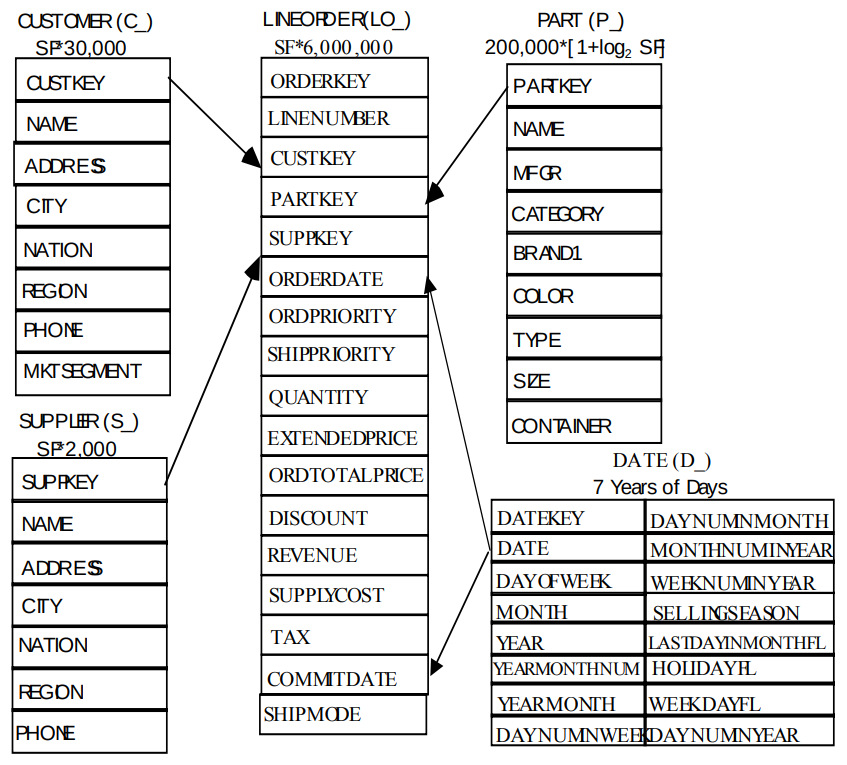
\includegraphics[width=1\textwidth]{pictures/ssb/ssb-schema.png}
    \caption{Schema des \ac{SSB}~\cite{oneil_star_2009}}      % caption the image
    \label{pic:ssb-schema}    % label the image for internal referencing
\end{figure}


\subsubsection{Queries des \ac{SSB}}
Die Queries des \ac{SSB} unterscheiden sich von denen des \ac{TPC-H}.
Der \ac{SSB} nutzt nur Queries, die genau eine SELECT-Anweisung auf der Faktentabelle LINEORDER nutzen und somit keine self-joins nutzen. %self-joins bissl weirder Ausdruck
Die LINEORDER Tabelle wird dann mit einer oder mehreren Dimensionstabellen gejoint und die Ergebnisse somit gefiltert. 
%TODO: Alle SSB SQL-Queries in den Anhang packen

Die Queries des \ac{SSB} sind in vier Kategorien aufgeteilt (query flights): % query flights bissl weird

%TODO: \usepackage{underscore}

\paragraph{Q1}
%ausbauen
Queries in Q1 schränken die Daten über nur eine Dimension, DATE, ein.
Die Faktentabelle LINEORDER wird mit der Dimensionstabelle DATE gejoint und die Daten anhand einer Zeitspanne aus der DATE-Tabelle und den Bereichen der Felder lo\_discount und lo\_quantity aus der LINEORDER-Tabelle gefiltert.
Anschließend wird der Umsatz als Summe der Produkte der Felder lo\_extendedprice und lo\_discount berechnet und als "revenue" zurückgegeben \cite{oneil_star_2009}.


\begin{lstlisting}[
    language=SQL,
    caption=SQL Query-Struktur für Q1 des \ac{SSB},
    label=code:ssb-q1-structur-example
]
SELECT 
    SUM(lo_extendedprice * lo_discount) AS revenue
FROM 
    lineorder, date
WHERE 
    lo_orderdate = d_datekey
    AND d_year = [YEAR]
    -- Specific values below
    AND lo_discount BETWEEN [DISCOUNT] - 1 AND [DISCOUNT] + 1
    AND lo_quantity < [QUANTITY];
\end{lstlisting}

\paragraph{Q2}
In Q2 schränken die Queries die Daten über zwei Dimensionen ein: PART und SUPPLIER.
Anschließend wird wie in Q1 der Umsatz gebildet, wobei die Ergebnisse hier noch nach d\_year und p\_brand1 gruppiert und sortiert werden.  
In Q2 werden insgesamt vier Tabellen (LINEORDER, PART, SUPPLIER, DATE) gejoint.
\begin{lstlisting}[
    language=SQL,
    caption=SQL Query-Struktur für Q2 des \ac{SSB},
    label=code:ssb-q2-structur-example
]
SELECT 
    SUM(lo_revenue) AS total_revenue, d_year, p_brand1
FROM 
    lineorder, date, part, supplier
WHERE 
    lo_orderdate = d_datekey
    AND lo_partkey = p_partkey
    AND lo_suppkey = s_suppkey
    AND p_category = 'MFGR#12'
    AND s_region = 'AMERICA'
GROUP BY 
    d_year, p_brand1
ORDER BY 
    d_year, p_brand1;

\end{lstlisting}

\paragraph{Q3}
In Q3 schränken die Queries die Daten über drei Dimensionen ein: DATE, SUPPLIER und CUSTOMER.
Wie in Q1 und Q2 werden auch hier die Umsätze gebildet.
Anschließend werden sie nach c\_nation, s\_region und d\_year gruppiert und nach d\_year sortiert.
Es werden insgesamt vier Tabellen (LINEORDER, DATE, SUPPLIER und CUSTOMER) gejoint.
\begin{lstlisting}[
    language=SQL,
    caption=SQL Query-Struktur für Q3 des \ac{SSB},
    label=code:ssb-q3-structur-example
]
SELECT 
    c_nation, s_nation, d_year, SUM(lo_revenue) AS revenue
FROM 
    customer, lineorder, supplier, date
WHERE 
    lo_custkey = c_custkey
    AND lo_suppkey = s_suppkey
    AND lo_orderdate = d_datekey
    AND c_region = 'ASIA'
    AND s_region = 'ASIA'
    AND d_year >= 1992
    AND d_year <= 1997
GROUP BY 
    c_nation, s_nation, d_year
ORDER BY 
    d_year ASC, revenue DESC;
\end{lstlisting}

\paragraph{Q4}
Die Queries von Q4 schränken die Daten basierend auf drei Dimensionen (CUSTOMER, SUPPLIER und PART) ein.
Auch hier wird wieder der Umsatz berechnet.
Dieses Mal wird er durch d\_year und c\_nation gruppiert und sortiert.
Hier werden erstmals alle fünf Tabellen (LINEORDER, CUSTOMER, SUPPLIER, PART und DATE) gejoint.
\begin{lstlisting}[
    language=SQL,
    caption=SQL Query-Struktur für Q4 des \ac{SSB},
    label=code:ssb-q4-structur-example
]
SELECT 
    d_year, c_nation, SUM(lo_revenue - lo_supplycost) AS profit
FROM 
    date, customer, supplier, part, lineorder
WHERE 
    lo_custkey = c_custkey
    AND lo_suppkey = s_suppkey
    AND lo_partkey = p_partkey
    AND lo_orderdate = d_datekey
    AND c_region = 'AMERICA'
    AND s_region = 'AMERICA'
    AND (p_mfgr = 'MFGR#1' OR p_mfgr = 'MFGR#2')
GROUP BY 
    d_year, c_nation
ORDER BY 
    d_year, c_nation;

\end{lstlisting}
\section{Redis}

Redis ist ein Key-Value Store, der vollständig im Arbeitsspeicher (in-memory) arbeitet und heute häufig als Datenbank, Cache, Message Broker oder Streaming Engine eingesetzt wird~\cite{redis_introduction_nodate}.
In Redis können unterschiedliche Datenstrukturen verwendet werden. Dazu gehören Strings, Hashes, Listen, Sets, sortierte Sets, Bitmaps, Hyperloglogs, georäumliche Indizes und Streams.
Mit Erweiterungen, so genannten Modulen, können weitere Datentypen wie z.B. JSON unterstützt werden.
Redis wird von vielen bekannten Unternehmen wie GitHub, StackOverflow, Snapchat, Craigslist oder X verwendet~\cite{redis_whos_nodate}.

\section{Scala}
% TODO: ganz kurzes Kapitel über Scala bzw. warum Scala